\documentclass{article}
\usepackage{fullpage}
\usepackage{nopageno}
\usepackage{amsmath}
\usepackage{graphicx}
\allowdisplaybreaks

\newcommand{\abs}[1]{\left\lvert #1 \right\rvert}
\newcommand{\degree}{\ensuremath{^\circ}}

\begin{document}
Jon Allen

HW 16

Lesson 10 exercise 3. Find the cosine transform $U(\omega ,t)$ of the solution $u(x,t)$

Solve by means of the sine \emph{or} cosine transform
\begin{align*}
  \text{PDE}&&u_t&=\alpha ^2u_{xx}&0<&x<\infty\\
  \text{BC}&&u_x(0,t)&=0&0<&t<\infty\\
  \text{IC}&&u(x,0)&=H(1-x)&0\le&x<\infty
\end{align*}
where $H(x)$ is the \emph{Heaviside function}:
\begin{align*}
  H(x)&=
  \begin{cases}
    0&0\le x<1\\
    1&1\le x
  \end{cases}
\end{align*}
\emph{Note:} The text is wrong. The above is actually the function $H(1-x)$ not the function $H(x)$.

%In other words, the IC looks like this
%\begin{center}
%  % GNUPLOT: LaTeX picture with Postscript
\begingroup
  \makeatletter
  \providecommand\color[2][]{%
    \GenericError{(gnuplot) \space\space\space\@spaces}{%
      Package color not loaded in conjunction with
      terminal option `colourtext'%
    }{See the gnuplot documentation for explanation.%
    }{Either use 'blacktext' in gnuplot or load the package
      color.sty in LaTeX.}%
    \renewcommand\color[2][]{}%
  }%
  \providecommand\includegraphics[2][]{%
    \GenericError{(gnuplot) \space\space\space\@spaces}{%
      Package graphicx or graphics not loaded%
    }{See the gnuplot documentation for explanation.%
    }{The gnuplot epslatex terminal needs graphicx.sty or graphics.sty.}%
    \renewcommand\includegraphics[2][]{}%
  }%
  \providecommand\rotatebox[2]{#2}%
  \@ifundefined{ifGPcolor}{%
    \newif\ifGPcolor
    \GPcolorfalse
  }{}%
  \@ifundefined{ifGPblacktext}{%
    \newif\ifGPblacktext
    \GPblacktexttrue
  }{}%
  % define a \g@addto@macro without @ in the name:
  \let\gplgaddtomacro\g@addto@macro
  % define empty templates for all commands taking text:
  \gdef\gplbacktext{}%
  \gdef\gplfronttext{}%
  \makeatother
  \ifGPblacktext
    % no textcolor at all
    \def\colorrgb#1{}%
    \def\colorgray#1{}%
  \else
    % gray or color?
    \ifGPcolor
      \def\colorrgb#1{\color[rgb]{#1}}%
      \def\colorgray#1{\color[gray]{#1}}%
      \expandafter\def\csname LTw\endcsname{\color{white}}%
      \expandafter\def\csname LTb\endcsname{\color{black}}%
      \expandafter\def\csname LTa\endcsname{\color{black}}%
      \expandafter\def\csname LT0\endcsname{\color[rgb]{1,0,0}}%
      \expandafter\def\csname LT1\endcsname{\color[rgb]{0,1,0}}%
      \expandafter\def\csname LT2\endcsname{\color[rgb]{0,0,1}}%
      \expandafter\def\csname LT3\endcsname{\color[rgb]{1,0,1}}%
      \expandafter\def\csname LT4\endcsname{\color[rgb]{0,1,1}}%
      \expandafter\def\csname LT5\endcsname{\color[rgb]{1,1,0}}%
      \expandafter\def\csname LT6\endcsname{\color[rgb]{0,0,0}}%
      \expandafter\def\csname LT7\endcsname{\color[rgb]{1,0.3,0}}%
      \expandafter\def\csname LT8\endcsname{\color[rgb]{0.5,0.5,0.5}}%
    \else
      % gray
      \def\colorrgb#1{\color{black}}%
      \def\colorgray#1{\color[gray]{#1}}%
      \expandafter\def\csname LTw\endcsname{\color{white}}%
      \expandafter\def\csname LTb\endcsname{\color{black}}%
      \expandafter\def\csname LTa\endcsname{\color{black}}%
      \expandafter\def\csname LT0\endcsname{\color{black}}%
      \expandafter\def\csname LT1\endcsname{\color{black}}%
      \expandafter\def\csname LT2\endcsname{\color{black}}%
      \expandafter\def\csname LT3\endcsname{\color{black}}%
      \expandafter\def\csname LT4\endcsname{\color{black}}%
      \expandafter\def\csname LT5\endcsname{\color{black}}%
      \expandafter\def\csname LT6\endcsname{\color{black}}%
      \expandafter\def\csname LT7\endcsname{\color{black}}%
      \expandafter\def\csname LT8\endcsname{\color{black}}%
    \fi
  \fi
  \setlength{\unitlength}{0.0500bp}%
  \begin{picture}(7200.00,5040.00)%
    \gplgaddtomacro\gplbacktext{%
      \csname LTb\endcsname%
      \put(726,440){\makebox(0,0)[r]{\strut{}-0.5}}%
      \put(726,1524){\makebox(0,0)[r]{\strut{} 0}}%
      \put(726,2608){\makebox(0,0)[r]{\strut{} 0.5}}%
      \put(726,3691){\makebox(0,0)[r]{\strut{} 1}}%
      \put(726,4775){\makebox(0,0)[r]{\strut{} 1.5}}%
      \put(858,220){\makebox(0,0){\strut{} 0}}%
      \put(2047,220){\makebox(0,0){\strut{} 2}}%
      \put(3236,220){\makebox(0,0){\strut{} 4}}%
      \put(4425,220){\makebox(0,0){\strut{} 6}}%
      \put(5614,220){\makebox(0,0){\strut{} 8}}%
      \put(6803,220){\makebox(0,0){\strut{} 10}}%
    }%
    \gplgaddtomacro\gplfronttext{%
      \csname LTb\endcsname%
      \put(5816,4602){\makebox(0,0)[r]{\strut{}h(1-x)}}%
    }%
    \gplbacktext
    \put(0,0){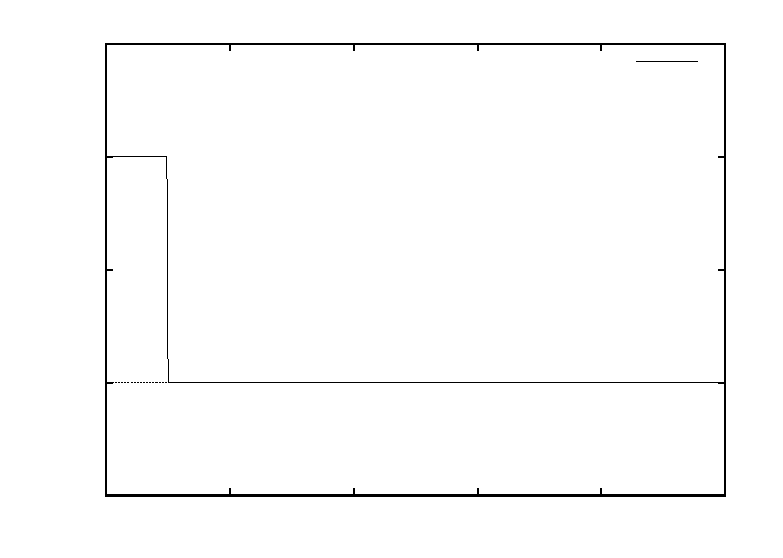
\includegraphics{pde-hw-16-plot-01}}%
    \gplfronttext
  \end{picture}%
\endgroup

%\end{center}

\begin{align*}
  \mathcal{F}_c[u_t]&=\alpha ^2\mathcal{F}_c[u_{xx}]\\
  \mathcal{F}_c[u_t]&=\frac{2}{\pi }\int_0^\infty{u_t\cos(\omega x)\,\mathrm{d}x}&
  \mathcal{F}_c[u_{xx}]&=\frac{2}{\pi }\int_0^\infty{u_{xx}\cos(\omega x)\,\mathrm{d}x}\\
  &=\frac{\partial}{\partial t}\left[\frac{2}{\pi }\int_0^\infty{u\cos(\omega x)\,\mathrm{d}x}\right]&
  &=-\frac{2}{\pi }{u_x}'(0,t)-\omega^2\mathcal{F}_c[u]\\
  &=\frac{\mathrm{d}}{\mathrm{d}t}\mathcal{F}_c[u]=\frac{\mathrm{d}}{\mathrm{d}t}U(t)&
  &=-\omega^2U(t)\\
  \frac{\mathrm{d}U}{\mathrm{d}t}&=\alpha^2\left[-\omega^2U(t)\right]&
  \mathcal{F}_c[u(x,0)]&=\frac{2}{\pi }\int_0^\infty{H(1-x)\cos(\omega x)\,\mathrm{d}x}\\
  U'+\omega^2\alpha^2U&=0
  &&=\frac{2}{\pi }\int_0^1{\cos(\omega x)\,\mathrm{d}x}\\
  \mu &=e^{\int{(\omega \alpha )^2\,\mathrm{d}t}}
  &&=\frac{2}{\pi }\left[\frac{\sin(\omega x)}{\omega }\right]_0^1\\
  &=e^{(\omega \alpha )^2t}
  &U(0)&=\frac{2}{\pi }\frac{\sin(\omega )}{\omega }\\
  e^{\omega^2 \alpha^2t}U&=\int{0\,\mathrm{d}t}&
  U(t)&=c_1e^{-\omega ^2\alpha^2t}\\
  U(0)&=c_1e^0=c_1=\frac{2}{\pi }\frac{\sin(\omega )}{\omega }&
  U(t)&=\frac{2}{\pi }\frac{\sin(\omega )}{\omega }e^{-\omega ^2\alpha^2t}\\
\end{align*}
\end{document}
